\chapter{Methodology}

This chapter fully explores the design of the experimental study, including the participant cohorts, the activities they performed, and the curricular context surrounding them. Also discussed in detail are the systems that were developed to support the study.

Data were collected from students working in classroom and summer camp programming activities in App Inventor. These data consisted of in-progress snapshots of their projects, where every change to an app was captured for every student. This chapter describes the study in general, the data collection system, the nature of the data collected, the programming activities the students were conducting.


\section{The Experiment}

The study consisted of two small programming challenges, where students were given a constrained programming problem. Their work on those problems were recorded using the snapshot system.

\subsection{Participant Selection \& Recruitment} 

All participants were from an ongoing project, \emph{Middle School Pathways in Computer Science,} a partnership between the University of Massachusetts Lowell, the urban school districts of Medford and Everett, MA, and the Tri-City Technology Education Collaborative Inc. This project developed and implemented in-school and summer camp curricula in mobile app development using App Inventor, centralized around ``Computing with a Community Focus'' \citep{Ni-2016}. The in-classroom implementations of this program ``infused'' programming into existing curricula. Teachers used their existing courses and learning goals as framing for the programming content. \label{sec:infusion} The summer camp implementations focused on app development, but did so with framing around solving local community problems.

Six cohorts participated. Four cohorts were from formal, in-school classes, and two were from informal summer camp environments. The total number of participants was 127, which is broken out into cohorts in Table \ref{tab:cohorts}.

Teachers of the in-classroom program who had at least one whole year of experience with the program were asked to volunteer a class period for this experiment. From the volunteered classes, three were selected based on schedule availability. A fourth in-classroom cohort was added when one teacher requested that researchers return to run the activity again with an additional class section.

\begin{table}
\begin{centering}
	\begin{tabular}{clr}
	Cohort & Environment & $n$ \\
	\hline
	1 & Classroom & 21		\\
	2 & Classroom & 24		\\
	3 & Classroom & 20		\\
	4 & Classroom & 21		\\
	5 & Summer Camp & 22	\\
	6 & Summer Camp & 19	\\ \hline
	\multicolumn{2}{r}{Classroom Total} & 86 \\
	\multicolumn{2}{r}{Summer Camp Total} & 41 \\ \hline \hline
	\multicolumn{2}{r}{\textbf{Total Participants}} & \textbf{127} \\ 
	
	\end{tabular}
	\caption[Participant Cohorts]{Participant cohorts, their environments in which the activities were conducted, and the number of participants for each.}
	\label{tab:cohorts}
\end{centering}
\end{table}


\subsection{Session Protocol}
The programming activities served as embedded assessment instruments. To begin, a researcher gave a brief introduction to the concept behind the activity, including making the learning outcome explicit to the students. Each activity consisted of an unfinished App Inventor project for the students to complete, and a paper worksheet for the student to document their work. 

The Debugging Activity provided an app similar to one the students (largely) had previously worked on, with instructions to fix mistakes in it. During the school year sessions, the activity was integrated by the teachers to fit in their curriculum (Section \ref{sec:infusion}). The Temperature Activity provided a Celsius/Fahrenheit unit converter app, missing the mathematical expression of the conversion, with instructions for the students to fill in that expression. The temperature activity was only run during the summer camp. The debugging activity was run in formal classrooms and during the summer camp. All activities were allotted a time frame of 30 minutes. During in-class sessions, which each consumed a 40-minute class period, approximately 10 minutes were necessary for classroom management and equipment distribution, so the 30-minute activity fit well. 

%Starting approximately halfway through the 30-minute period, researchers were allowed to begin giving hints to students who appeared stuck, and were trained on giving the same set of hints in all instances. The hints were limited to pointing out where the interesting class of block resided in the UI, re-reading questions aloud to promote deeper engagement, and only in the last few minutes, active guidance. 

%The students each were given a worksheet that had a special URL that they typed into their browsers. That URL delivered them to the instrumented version of App Inventor, and automatically inserted the starter file into their account, and opened it for use. The students then had up to 30 minutes to solve the tasks and answer the questions on the worksheet. The students were given tablets, enabling live testing throughout the activity. 


\subsection{The Debugging Activity}
All cohorts participated in the debugging activity. The protocol included a short slide show presentation, with interactive questions for the students, to scaffold the idea of debugging and frame the student's assigned task. The scaffolding presentation, description of the starter app, and copy of the worksheet are included in Appendix \ref{apx:debugging-protocol}.

\begin{figure}
  \centering
      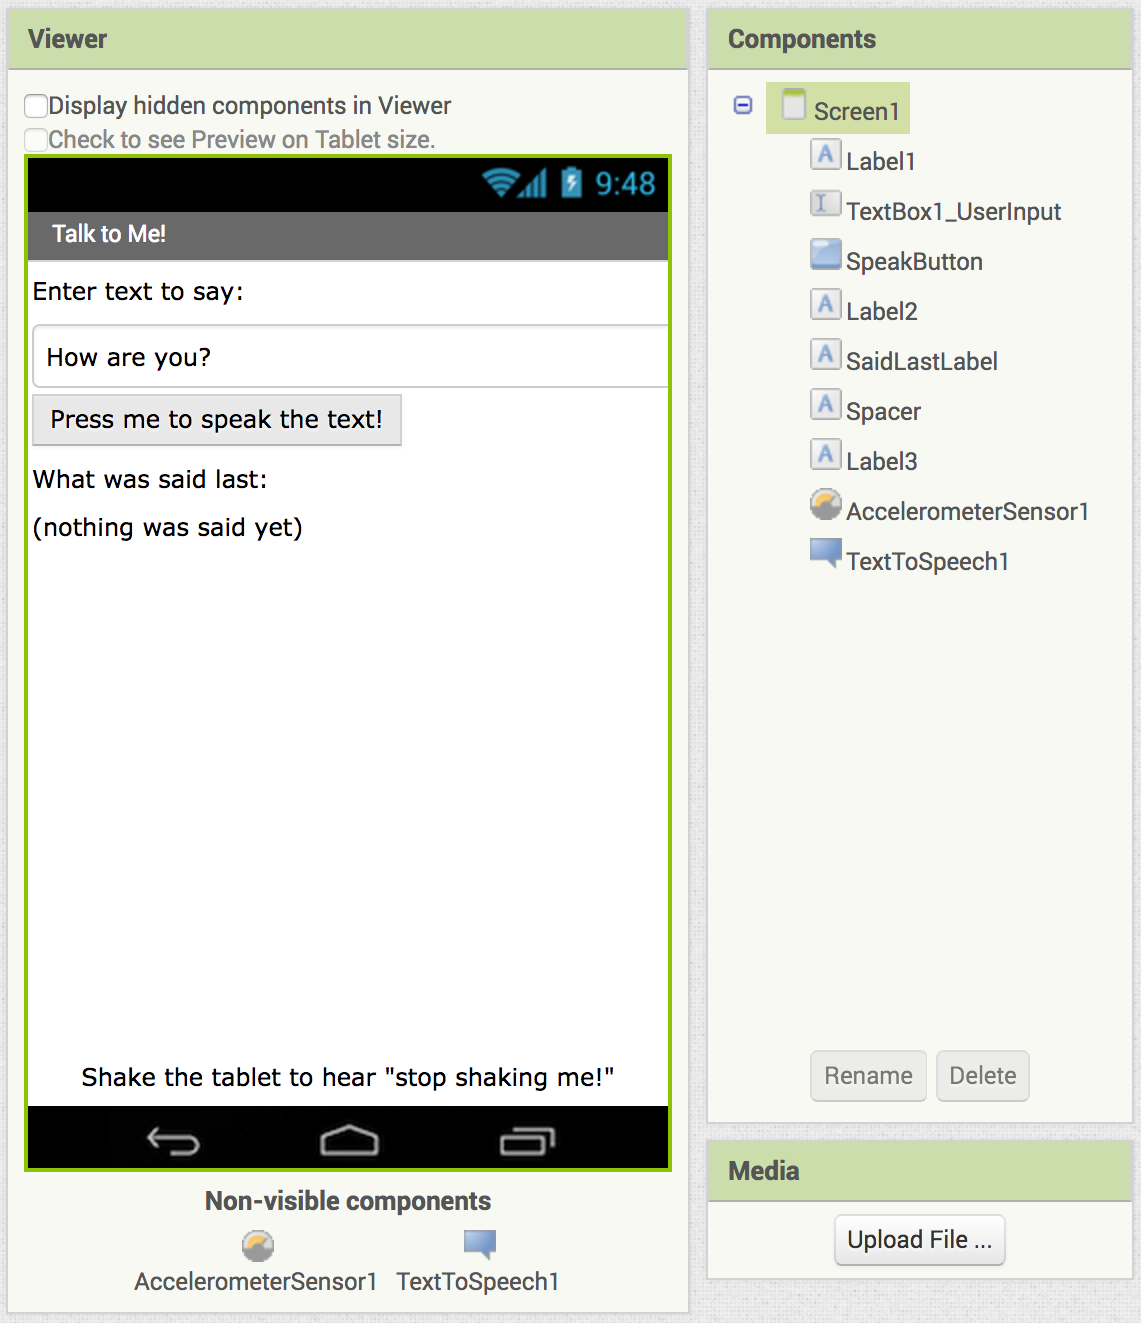
\includegraphics[width=\textwidth]{images/debugActivity/debug-designer}
  \caption[The Debugging Activity Designer View]{The Debugging Activity app screen in the App Inventor designer.}
  \label{fig:debug-screen}
\end{figure}

The app was a variant of \emph{TalkToMe,} a common introductory project with App Inventor. All of the students in the summer camp cohorts, and most of the students in the classroom cohorts, had seen \emph{TalkToMe} prior to this activity. The activity design did not require this prerequisite experience, and there was no visible difference in performance among the few students who did not have it. The app's screen design is shown in Figure \ref{fig:debug-screen}, and the starting state of the code blocks is shown in Figure \ref{fig:debug0}.

\begin{figure}
  \centering
      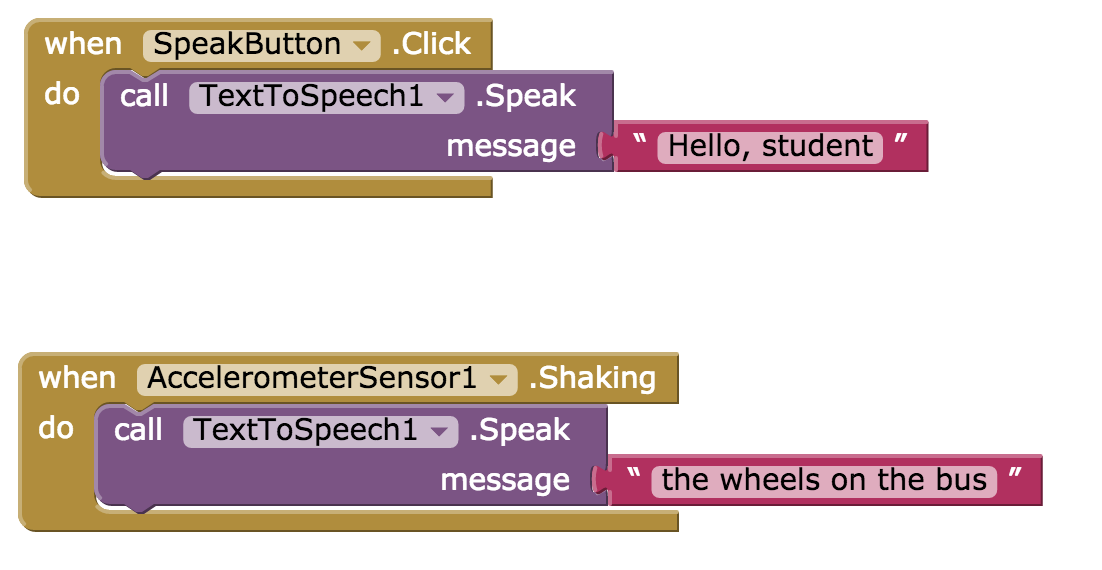
\includegraphics[width=\textwidth]{images/debugActivity/debug0start}
  \caption[The Debugging Activity Starter Code Blocks]{The Debugging Activity starter code blocks. Note that neither text matches the description on the screen in Figure \ref{fig:debug-screen}.}
  \label{fig:debug0}
\end{figure}


The app had three bugs, presented in ascending order of difficulty. The students were instructed not to change any components of the design of the app. Their changes were only to be limited to the code blocks. The screen design could be used as a source of information to infer what the app was supposed to do, which was important in identifying and correcting the bugs. The bugs were:

\begin{enumerate}
\item Mismatch between label ``stop shaking me!'' and the actual spoken text when shaken, ``the wheels on the bus.''
\item Mismatch between what is in the text input box and what was spoken when the button is pressed.
\item ``What was said last'' did not update as expected.
\end{enumerate}

The first bug was easily solved by changing the text literal from ``the wheels on the bus'' to ``stop shaking me,'' as seen in Figure \ref{fig:debug1}. The second bug was more nuanced. In preliminary work with this instrument, we discovered that there were two degrees of understanding within the second bug. In the first degree solution, the student modified the text literal within the button click event to match the text on the screen, in effectively the same fashion as the first bug (also shown in Figure \ref{fig:debug1}). This solution made the second bug appear solved, but only superficially. The second degree solution required the realization that the input box could be changed, and the text to be spoken needed to reference that box as a variable in order to always say the correct text. This concept was modeled in the previous exposure to the \emph{Talk To Me} app. The solution involved recruiting a new block into the workspace, the input box's contents reference, and replacing the static text with that reference block. This solution is shown in Figure \ref{fig:debug2}. Making the realization and recruiting the additional block to execute it made this solution more challenging.

\begin{figure}
  \centering
      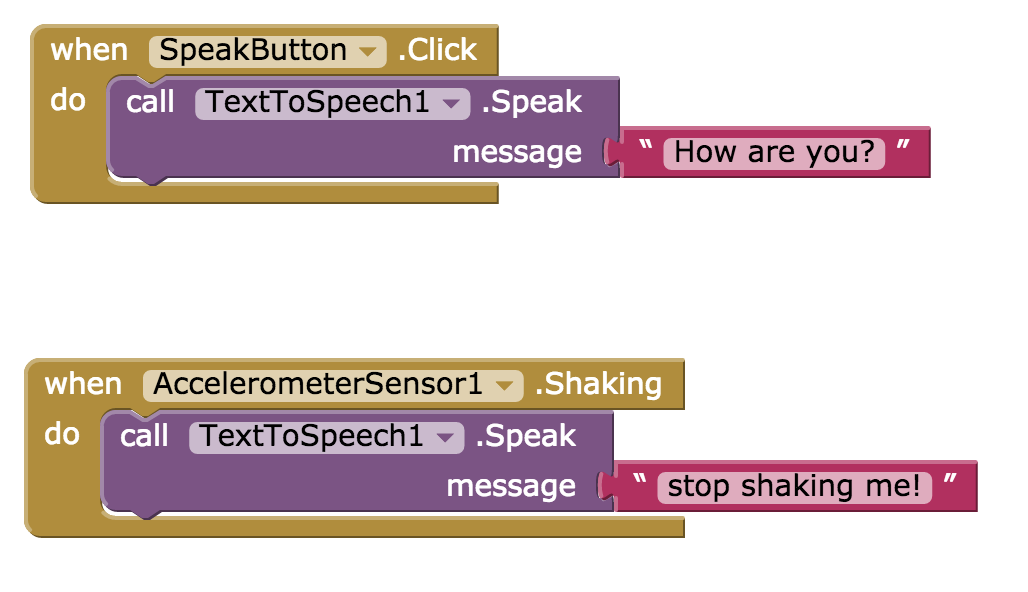
\includegraphics[width=\textwidth]{images/debugActivity/debug1shaking}
  \caption[First Degree Solutions to the Second Bug]{First degree solution to the second bug, speaking user inputted text, where the app always says ``How are you?'', and the shaking action always says ``stop shaking me.''}
  \label{fig:debug1}
\end{figure}

\begin{figure}
  \centering
      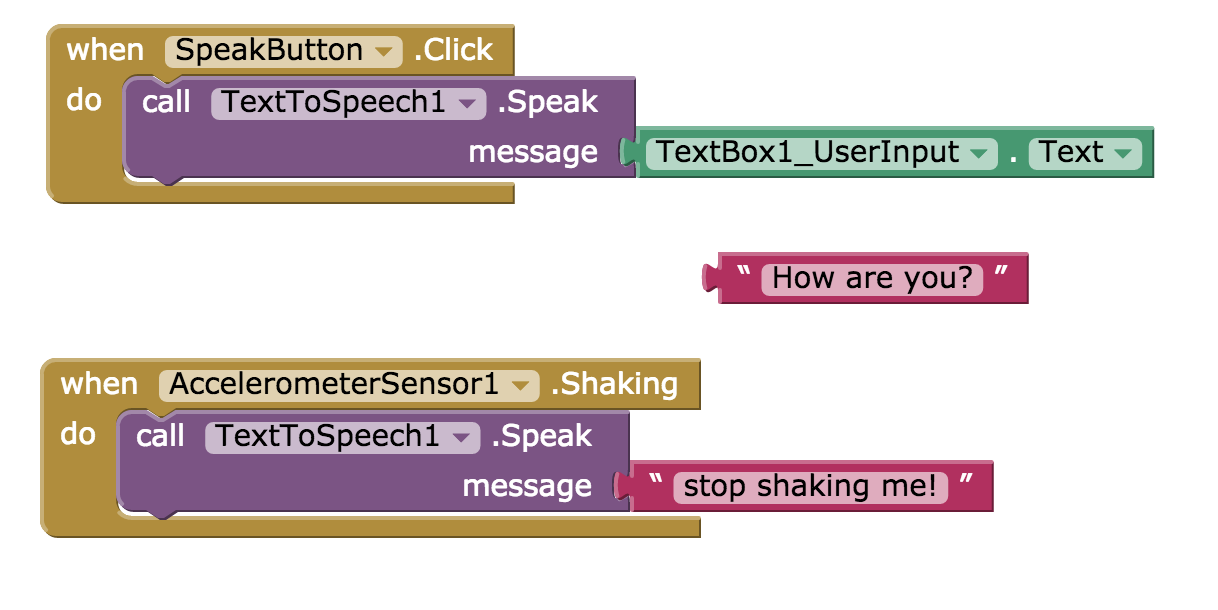
\includegraphics[width=\textwidth]{images/debugActivity/debug2input}
  \caption[Second Degree Solution to the Second Bug]{Second degree solution to the second bug, speaking user inputted text, where the user input text box is referenced like a variable. The previous text constant is shown as discarded to the side.}
  \label{fig:debug2}
\end{figure}

\begin{figure}
  \centering
      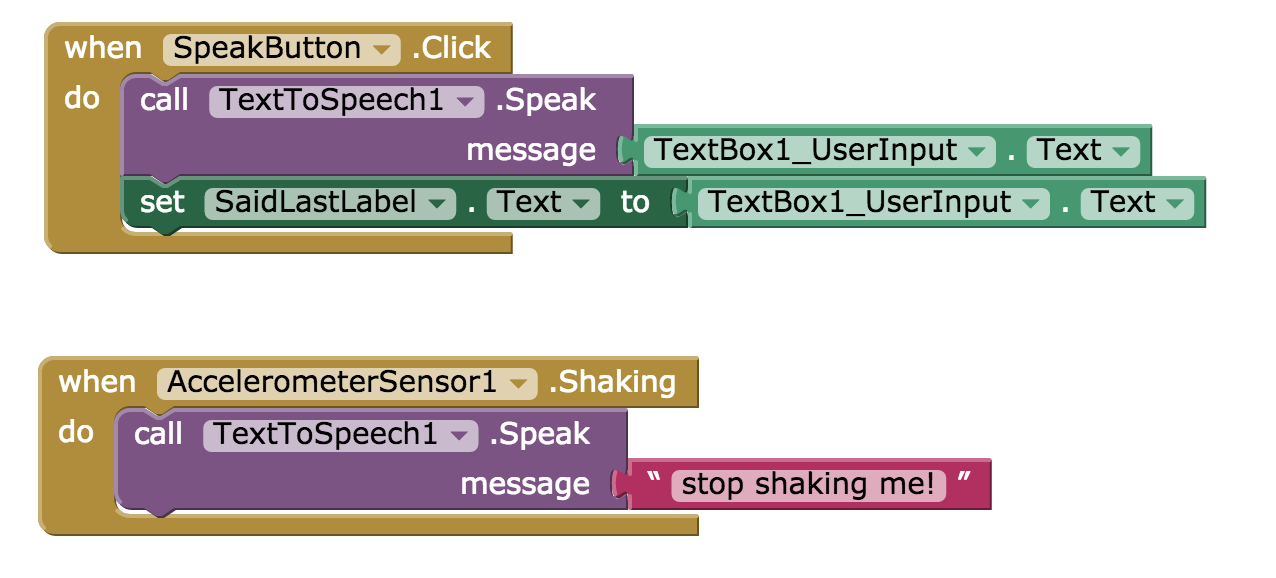
\includegraphics[width=\textwidth]{images/debugActivity/debug3saidlast}
  \caption[Solution to the Final Bug]{Solution to the third bug and final bug, which required storing the inputted text into a label as well as speaking it aloud.}
  \label{fig:debug3}
\end{figure}

The third bug was the most difficult, and was based on storing data to a label component. It involved adding an additional \emph{set} block to one of the existing event handlers, which required deeper understanding than the previous two bugs did. The solution is shown in Figure \ref{fig:debug3}. Less than half of the students attempted to solve this bug.


\subsection{The Temperature Activity}

\begin{figure}
  \centering
      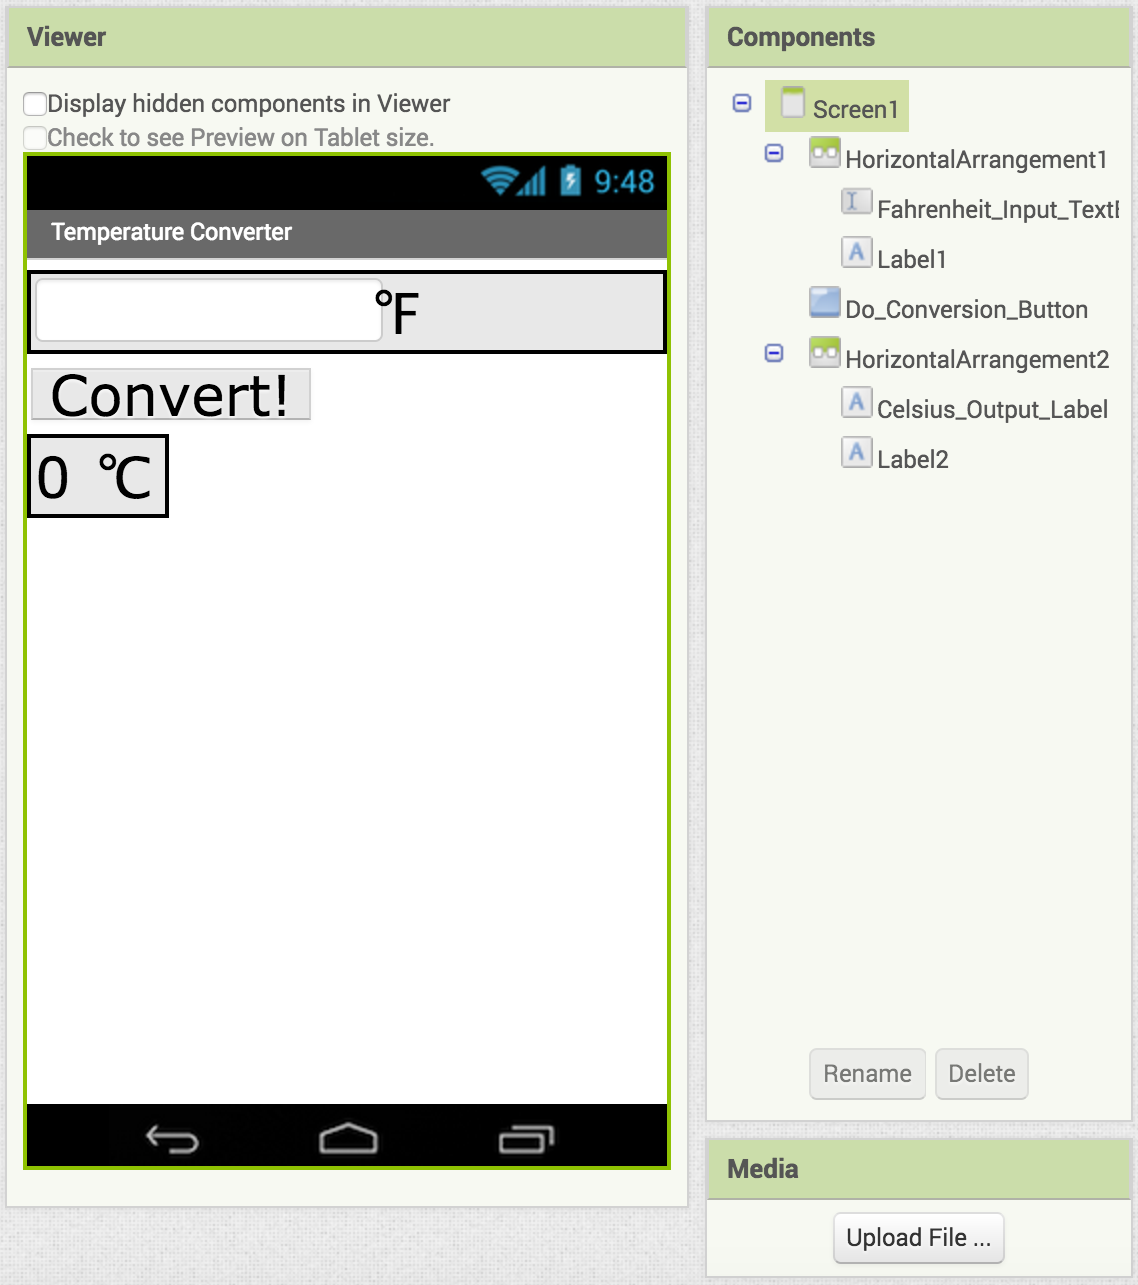
\includegraphics[width=\textwidth]{images/temperatureActivity/temperature-designer}
  \caption[Temperature Activity App Designer View]{The Temperature Activity app screen in the App Inventor designer.}
  \label{fig:temperature-screen}
\end{figure}

The temperature activity was designed to get students to construct a mathematical expression, by framing a need for a unit conversion. The screen design is shown in Figure \ref{fig:temperature-screen}. The starter app and worksheet are included in Appendix \ref{apx:temperature-protocol}. Only the summer camp cohorts participated in this activity. 

In this activity, students were given a one-way temperature converter. An input field was labeled as degrees F, and an output label was labeled as degrees C, with a button separating them labeled ``Convert!'' The blocks provided a procedure to carry out the numeric conversion from Fahrenheit to Celsius, and students were instructed only to modify that procedure. The starter code is shown in Figure \ref{fig:temperature0}.

This activity did not have the prior testing and validation that the debugging activity enjoyed. It needed improved scaffolding, as during execution of the activity most students struggled to understand what was being asked of them. Specifically, the instruction to only modify the conversion procedure was not well received, as it was not sufficiently clear how that procedure was supposed to be modified. Students largely did not understand that the value delivered to the \emph{result} socket represented the $C=$ part of the equation. But, serendipitously, this may provide researchers with a rich example set of flailing/progressing behavior. The solution is shown in Figure \ref{fig:temperature1}.

\begin{figure}
  \centering
      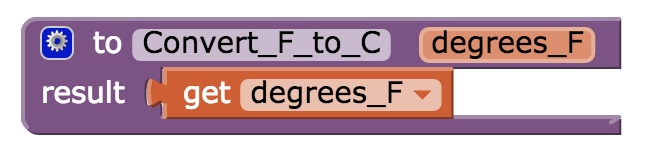
\includegraphics[width=3.6in]{images/temperatureActivity/temperature0start}
  \caption[Temperature Activity Starter Code Blocks]{The Temperature Activity starter code blocks.}
  \label{fig:temperature0}
\end{figure}

\begin{figure}
  \centering
      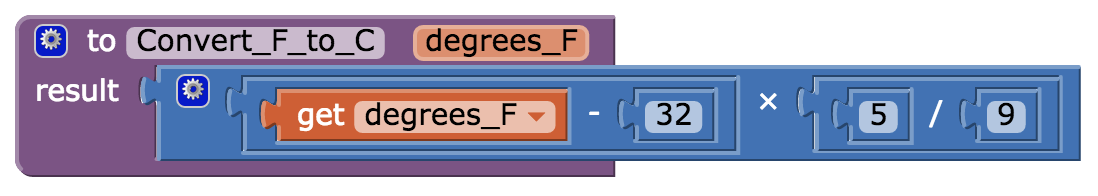
\includegraphics[width=\textwidth]{images/temperatureActivity/temperature1solution}
  \caption[Temperature Activity Solution]{The Temperature Activity solution.}
  \label{fig:temperature1}
\end{figure}



\section{The Data Collection System}
In order to carry out the study, instrumentation was built into App Inventor to collect rich student programming behavior data. As discussed, this instrumentation added to a growing tradition of instrumentation within the development environment itself, such as the works of \citet{berland-2013}, \citet{lipman-phd}, and others. The system collected a \emph{snapshot} on every change the user made to their app. With each snapshot, the entire contents of their source files (excluding media assets) were transmitted to a secure research server where they were de-identified and stored. This collection of snapshot data is the corpus from which relevant features were extracted for analysis.

\subsection{Snapshot Capture in App Inventor}
\label{sec:mod-ai}
Every time the user changed anything, for example: move a block, add a block, or modify a component, a snapshot was triggered, and the project state was captured. A single snapshot contained the entire block workspace and designer configuration in text form. Assets, including images uploaded, were not included. The basic architecture of the snapshot capture process is shown in Figure \ref{fig:snapshot-arch}.

\begin{figure}
  \centering
      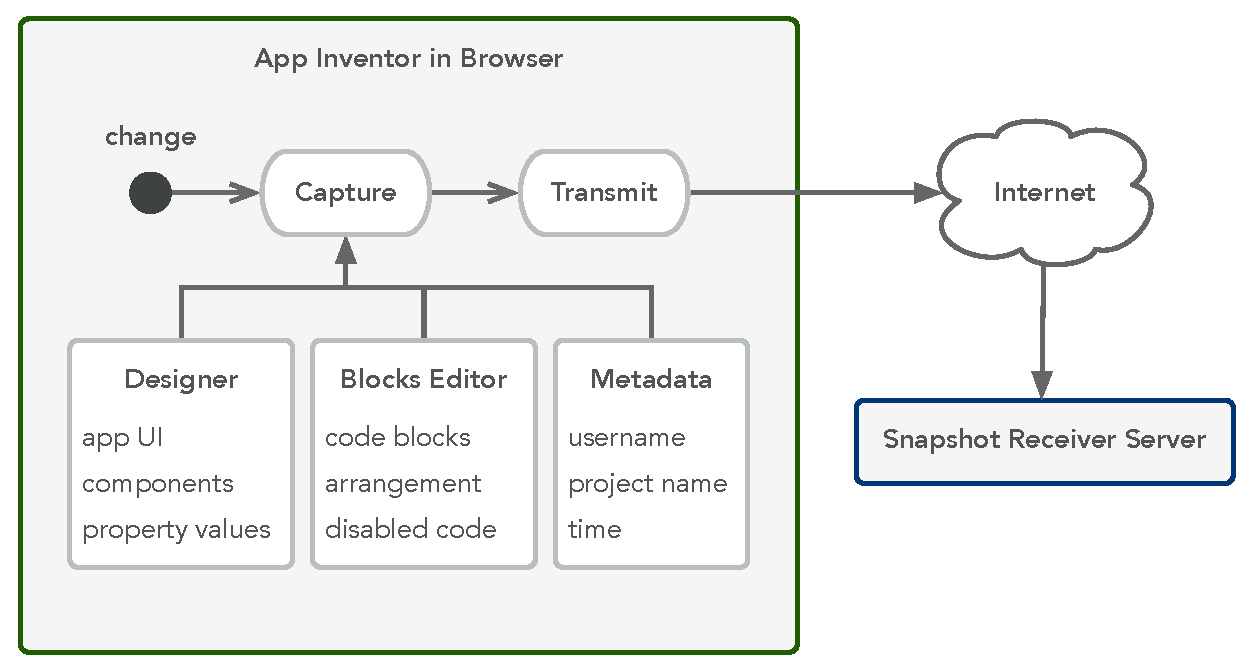
\includegraphics[width=\textwidth]{diagrams/architecture}
  \caption[Snapshot Capture Design Diagram]{The snapshot capture system in App Inventor, which is triggered by any change to blocks or designer. On a change, data from the designer, blocks editor, and additional metadata are captured and transmitted to the receiver server.}
  \label{fig:snapshot-arch}
\end{figure}

The snapshot payload was transmitted upon each user change to a server, where it was de-identified and stored. Details on the server's processes are below, in Section \ref{sec:server}. Additional technical detail on the implementation of the changes to App Inventor are below, in Section \ref{sub:tech:ai}.

\subsection{Snapshot Receiver Server}
\label{sec:server}
The snapshots captured in App Inventor were transmitted to a secure research server, running software that will be described in this section, and called the ``Snapshot Service.'' This server architecture received snapshot payloads from the custom instances of App Inventor, de-identified the user names, and stored the snapshots and metadata persistently. This service had to maintain the integrity of the sensitive, identifiable user data and reliably process peak load, which was tested up to hundreds of snapshots per second. The operation of the server is depicted in Figure \ref{fig:server-process}.


\begin{figure}
  \centering
      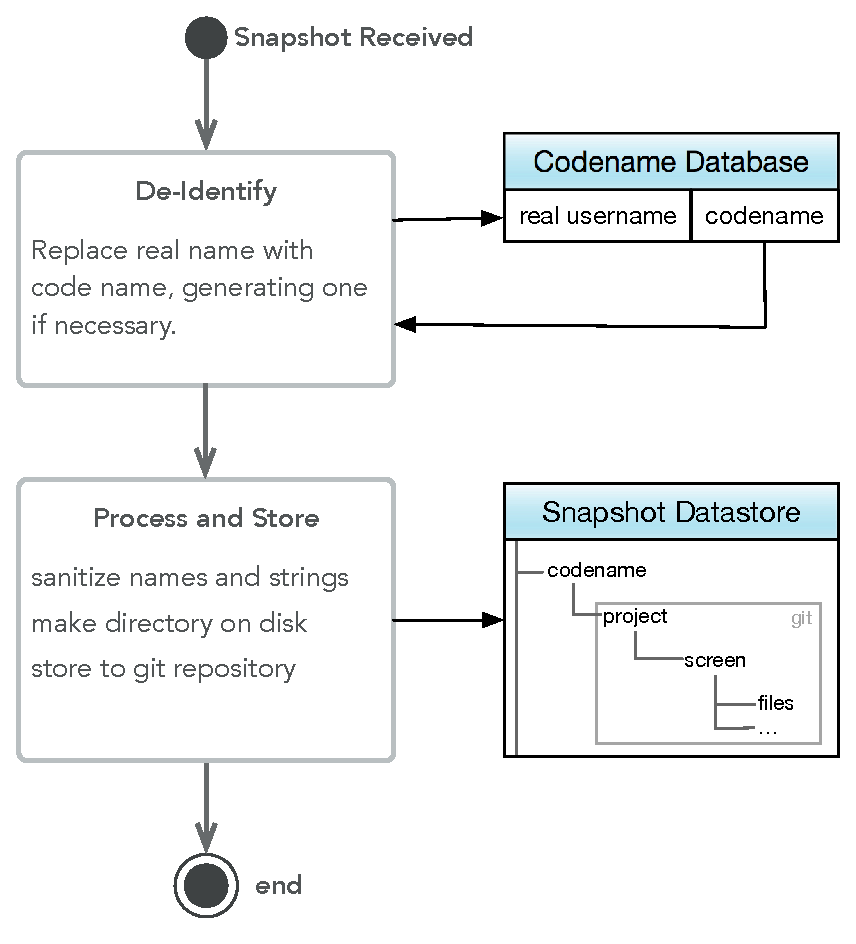
\includegraphics[width=\textwidth]{diagrams/server-operation}
  \caption[Server Operating Diagram]{Operating diagram for the snapshot collection server. The boxed folder ``project'' denotes the Git repository location.}
  \label{fig:server-process}
\end{figure}


\subsection{De-Identification}
\label{sec:deident}
Removal of identifiable user data is a critical issue in human subjects research. In accordance with the IRB approval, student work artifacts had to be stripped of identifiable information, and a system feature was implemented to do so automatically (Appendix \ref{IRB:deident}). This feature replaced the student's real user name with a randomized code name. This feature also kept record of the relations between real names and code names, allowing a consistent mapping. The same user would always be given the same code name, which was critical, as each snapshot was an addition to the data store. Without consistent user-to-codename mapping, the thousands of snapshots would be like a spilled deck of index cards, useless without order or consistency. 

The map between user names and code names was stored in a database file on the collection server. That server was only accessible to the author and two trusted IT personnel in the computer science department. Those IT personnel never accessed the server during the study period, or afterward, until the system was decommissioned. The database selected was sqlite3, because it uses a single, regular file as the data store that could be carefully controlled and protected. That file resided on the server, and was kept separate from the bulk snapshot data. The snapshot data could be moved and analyzed without fear of exposing the real names associated with those data. The mapping database file was only moved off the server in once instance, over encrypted and secured means, to the author's personal computer, which employed a reasonable guarantee of access control, like the server. This protocol was deemed safe by the research team and IRB.

Implementation of the de-identifier was conceptually straightforward: upon every snapshot, look up the user name in the database, and if found, replace the user name with the existing code name. If the user is not in the database, generate a new code name, and insert it into the database. Either way, a code name is returned, and replaces the user name. 

% In the event of an error, the entire snapshot save operation was aborted, so there was no possibility of data being saved without a valid, de-identified code name replacement. The de-identification system was thoroughly tested, protected with regression unit tests, and closely monitored during data collected. During the entire data collection, no error in this system occurred. The combination of sqlite3 and Node.js proved to be surprisingly fast, and handled the highest traffic periods with ease. The author would like to attribute this performance in part to their quality and efficient programming, but such cannot be validated scientifically at this time.

% The full source code of the de-identification module is in Appendix \ref{src:userdb.js}.

% \subsection{The Snapshot Database}
% \label{sec:db}
% The database containing the snapshot contents was a collection of Git directories. Each user project was a Git repository, and each recorded snapshot was a commit into that repository. Additional metadata was included in Git notes, or as a content file in the repository. This concept was based on the work of \citet{lipman-phd}. The technology of this database was differentiated by its enhanced granularity of data recorded, adoption of a remote client-server model, and future-looking adapters to allow use of different environments and different languages. The database itself was organized in directories on disk of the server, where the first level of directories contained users. Within each user folder were folders representing each project that was recorded for that user. The project names were a combination of the user-mutable project name and the unique project ID generated by App Inventor. The two fields were concatenated with a \emph{\#} character, which is not allowed in file names and does not occur in project IDs, so it provides a unique token to parse them apart, if needed. Within each project were directories for each screen. Most apps did not extend beyond the default screen, which is always called \emph{Screen1.} Within each screen folder were the contents of the designer and blocks, represented as JSON and XML files, respectively. This is visualized with example data in Table \ref{tab:Git-db-org}.

% \begin{table}
% \begin{centering}
% 	\begin{tabular}{ll}
% 	\hline
% 	DB directory&  \mintinline[fontsize=\footnotesize]{bash}{/}		\\
% 	Code name 	&  \mintinline[fontsize=\footnotesize]{bash}{/ColomboMoose}		\\
% 	Project name & \mintinline[fontsize=\footnotesize]{bash}{/ColomboMoose/JumpCount}		\\
% 	Project ID 	&  \mintinline[fontsize=\footnotesize]{bash}{/ColomboMoose/JumpCount#5743573328723968.Git}		\\
% 	Screen name	&  \mintinline[fontsize=\footnotesize]{bash}{/ColomboMoose/JumpCount#5743573328723968.Git/Screen1}		\\
% 	Blocks code	&  \mintinline[fontsize=\footnotesize]{bash}{/ColomboMoose/JumpCount#5743573328723968.Git/Screen1/blocks.xml}		\\
% 	Designer form& \mintinline[fontsize=\footnotesize]{bash}{/ColomboMoose/JumpCount#5743573328723968.Git/Screen1/form.json}		\\
% 	\hline
% 	\end{tabular}
% 	\caption[Organization of snapshot database.]{Organization of snapshot database, shown with example data, where each project was a Git repository, containing the whole contents of that project's code.}
% 	\label{tab:Git-db-org}
% \end{centering}
% \end{table}

% The primary benefit of using Git was that it allowed easy human perusal through the time line of projects, and provided code diffs for free. This feature set was briefly useful in assessing that the collection system was working, but in general, these benefits were not highly utilized. Analysis was conducted by developing python scripts to extract features from the data, leaving the human browsing features of Git irrelevant. The analysis tools are discussed in depth in Section \ref{sec:analysis-tools}. Additionally, this method of adding many commits to many Git repositories is disk-inefficient to Git itself, and resulted in an extremely large consumption rate of disk space, and more critically, file system inodes. Disk inodes are the handles that the file system uses to identify and find files, and the maximum number available on an ext4 file system is fixed. Working in this way, Git consumed an exorbitant number of these inodes, and required occasional repacking to free them, resulting in the development of the garbage collection script, included in Appendix \ref{src:gc.sh}. While the system was in use, that script needed to be run weekly to prevent the disk from filling and becoming unwritable. 

% \subsection{Engineering Concerns}
% Snapshots captured the entirety of the project's source text at every change. As a program was built, the number of blocks driving it was likely to grow, and the snapshot payload would grow linearly with it. This initially caused concern that the large block files could result in poor performance, such as: slowing down the student's browser, effecting their experience; slow transmission over school networks, creating incomplete or out-of-order snapshot data; or slowdown of the reception server, causing data to be lost or corrupted. In testing, these concerns were allayed. The system performed sufficiently fast under all test cases, indicating that, if possible, a truly extreme case would be necessary to adversely impact performance. The constraints of the experimental design inhibited such massive projects from developing.
% %TODO grab scary concerns from above sections and move them here for better clarity

\section{Technical Detail of Snapshot Collection}

The snapshot collection system started with modifications to App Inventor, which ran in the student's browser as their programming environment. These modifications collected the code states at every edit event, and transferred them to a server for de-identification and storage. 

\subsection{Implementation Details of App Inventor Modifications}
\label{sub:tech:ai}
App Inventor was primarily composed using the Google Web Toolkit (GWT), which allows rich web pages to be written in Java and compiled to HTML and JavaScript. Within the GWT-built App Inventor page, there is a panel hosting a somewhat-sandboxed Blockly environment, written in pure JavaScript. The snapshot mechanism was implemented in the Blockly environment, but required access to certain data in the GWT environment. The interface between GWT and Blockly was implemented in a file \mintinline{js}{BlocklyPanel.java}, which was modified to expose the necessary data. The \mintinline{js}{BlocklyPanel} file was large, with over a thousand lines in length, and governed the entire Blockly sandbox within App Inventor. Exposing new features to Blockly required adding new GWT Java methods to extract the data from the GWT-managed memory, and then adding corresponding JavaScript functions that would be exported into the Blockly environment that serve as wrappers for the GWT methods. 
%The modifications to this file, but not the file in its entirety, are listed in Appendix \ref{src:ai/BlocklyPanel.java}.

The snapshot mechanism itself was added to Blockly environment, and provided a single external function, \mintinline{js}{Blockly.Snapshot.send}. This function could be called anywhere from within Blockly (or within GWT, with some effort, if desired). In this experiment, snapshots were triggered in only one place, the REPL manager. The REPL manager maintained the connection between App Inventor and the connected target device. When a device was connected, any changes to the app in App Inventor were immediately sent to the device, all while the app continued to run on the device uninterrupted. The REPL manager made this possible, collecting code changes, compiling them, and sending them to the device. The snapshot send function was inserted into the REPL manager's \mintinline{js}{pollYail} routine, which was the function that was called to check if there was a code update to push to the phone. That function was called on-demand by the REPL manager anytime a change was made, with a small amount of change aggregation. That aggregation was intended to service the REPL in a good-enough fashion, which did not require changes to be updated on every pixel-wise change as a block was dragged across the screen, but did require the end position. This function already aggregated trivial, in-motion changes such as block dragging into atomic events, and this degree of granularity was ideal for snapshot capture. 

An alternative trigger point for snapshots was in the \mintinline{js}{blocklyWorkspaceChange} event callback function, but this position was overly aggressive, as it was used in the graphics engine of Blockly to repaint the screen on \emph{any} change. For a snapshot, in-progress block drags across the screen were considered part of the same atomic change. Only the final resting position was necessary for a the desired data density of a snapshot. Additionally, the workspace change event could be called hundreds of time more often than \mintinline{js}{pollYail,} which put unnecessary stress on the snapshot computation and transmission mechanisms. Triggering snapshots from within the REPL manager position, described above, offered an ideal compromise. Every logical block change was captured, but transient state of the block mid-change was not. Additionally, \mintinline{js}{pollYail} was also called in response to changes in the Designer, allowing component changes to trigger snapshots for free.

Another triggering option was considered, where each block type would have the trigger added to their modification callback functions, effectively instrumenting the individual blocks instead of the workspace as a whole. This option could have provided additional specificity, as it could reliably report the nature of the change that triggered the snapshot, such as ``text block was moved.'' The snapshot protocol was designed to accommodate such data, but was not utilized in this study. The engineering demand to implement this style of instrumentation with full coverage was too great to be complete in time for the study. As such, one weakness of the snapshot system as described here is that it does not know why a snapshot was triggered. That was traded for guarantee of full coverage, that no change would be missed. As a result, analysis required the construction of tools to extract that change data from the recorded data. Future work may include such event-driven metadata, and is further explored in Section \ref{sec:futurework}. The snapshot itself contained a collection of fields, shown in Table \ref{tab:snapshotPayload}. 

\begin{table}
\begin{centering}
	\begin{tabular}{l l}
		Data Field 			& Contents \\ \hline
		userName  			& User's real Google account name. \\
		projectName 		& User's project file name. 	\\
		projectId 			& Unique ID assigned to the project, invisible to user.	\\
		screenName 			& Which screen in the project the user is modifying.	\\
		sessionId 			& Browser session, to identify session boundaries in analysis.	\\
		yaversion 			& Current version of the App Inventor environment. 	\\
		languageVersion 	& Current version of the App Inventor blocks language. 	\\
		eventType 			& Future use: to explicitly identify the change event that occurred. 	\\
		blocks 				& Full content of the blocks, in XML. 	\\
		form 				& Full content of the screen's design, or form, in JSON.

	\end{tabular}
	\caption[Contents of a Snapshot]{The data contents of a single snapshot.}
	\label{tab:snapshotPayload}
\end{centering}
\end{table}

\subsection{Implementation Details of The Collection Server}
The server was written in Node.js \citep{nodejs}, a server-side JavaScript environment that provides high performance and reliability through an event-driven, asynchronous I/O model. %Relevant source code is included in Appendix \ref{src:snapshot-service}.

The service implemented a JSON-RPC API \citep{jsonrpc}, where each snapshot sent from App Inventor was a new RPC connection. There was one API endpoint, which accepted the data, applied the de-identifier, and dispatched the process to commit the change to disk. The RPC API, low-level system access, and Git access libraries, were based on similar technology developed by \citet{lipman-2011}. No part of that existing system was used wholesale, but the lessons learned from \citet{lipman-2014} strongly informed the design decisions presented here. Dr. \citeauthor{lipman-2014} also provided code review services for the present system. % The logic of the \mintinline{js}{saveProject} process was as follows:

% This is covered in slightly less detail above (better for reading). No need for this degree of specificity.
% \begin{enumerate}
% \item Parse JSON received from App Inventor
% \item Extract real user name from parsed data
% \item Replace real user name with code name (detail below in Section \ref{sec:deident})
% \item Save data to database:
% \begin{enumerate}
% 	\item Sanitize data, removing dangerous dots and slashes from filenames
% 	\item Assemble Git commit message
% 	\item Assemble directory for this project based on user code name and project ID
% 	\item Make directory on disk (using -p to only create new as required, preventing overwriting)
% 	\item Write files to directory (blocks and project form)
% 	\item Create Git repository in that directory (Git re-initializes non-destructively if it already exists)
% 	\item Set Git credentials for user, based on code name
% 	\item Stage and commit project files (blocks and project form)
% 	\item Amend current directory as Git notes
% \end{enumerate}
% \end{enumerate}


\section{Snapshot Playback}
\label{sec:playback}

A playback system was created to allow researchers to step through the snapshot history of any project. This system afforded the researchers the ability to load the entire history of a particular project, and easily walk through that history. The tool displayed the snapshot number (labeled as ``frame'', like a frame in a video), the time at which the snapshot occurred, and the interval time since the previous interval. 

%To start the playback mechanism, the researcher supplies the \emph{Playback.start} function of the modified version of App Inventor with a file name. The playback module looks for a local web server, fetches that file name, parses the JSON, and returns the control object. 
%The entirety of the module's source code is included in Appendix \ref{src:playback.js}. 
An example of the system at work is shown in Figure \ref{img:playback}. The controls are in the console at the bottom of the screen.

\begin{figure}
  \centering
      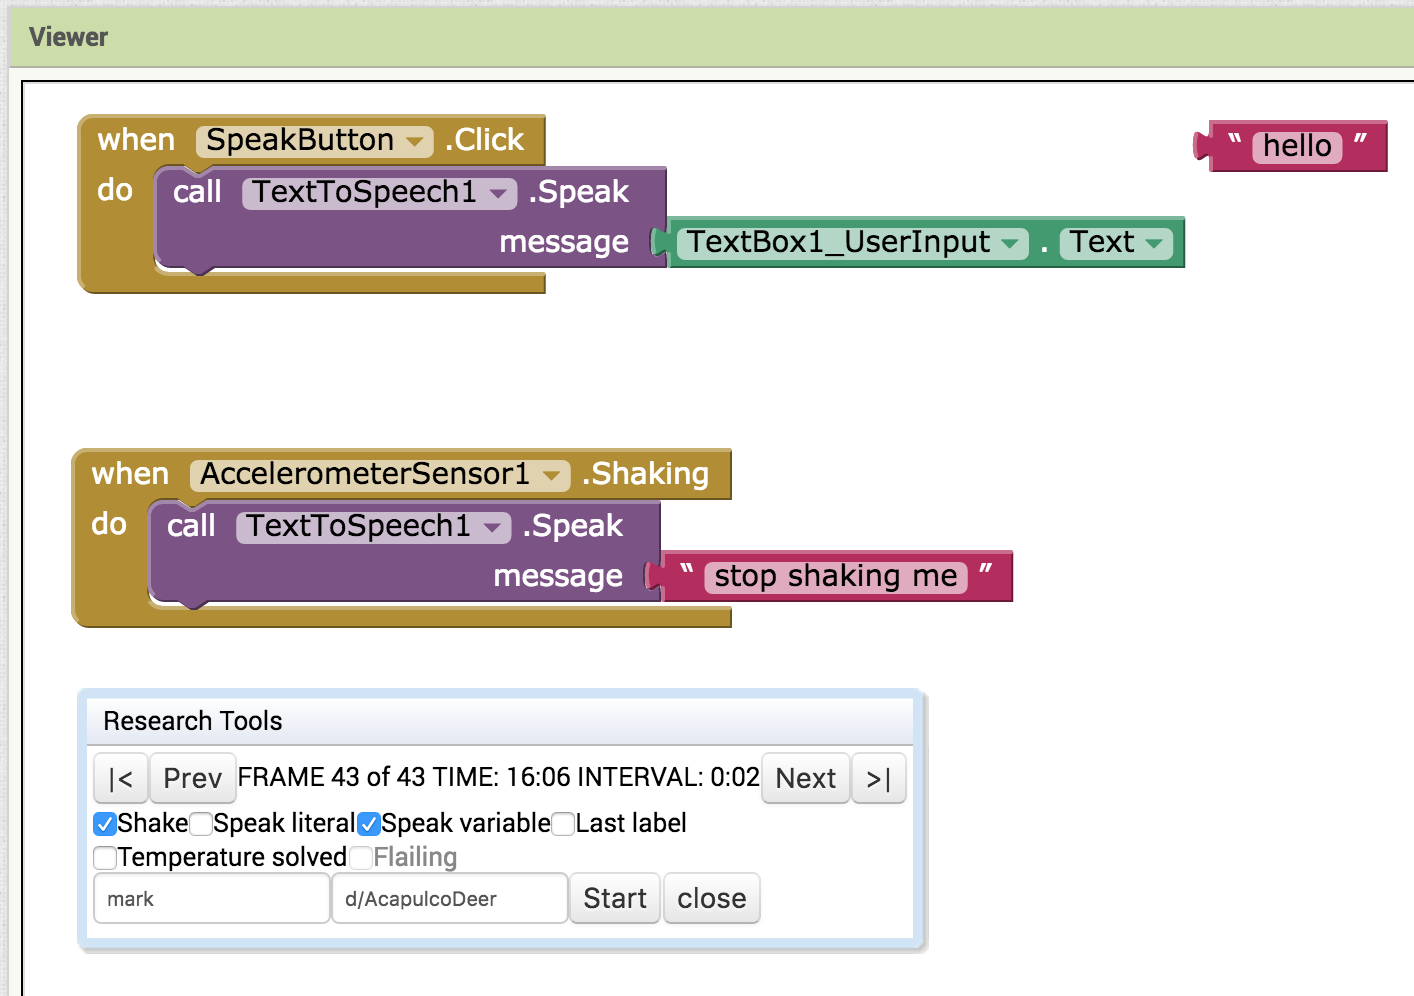
\includegraphics[width=\textwidth]{images/ch3-playback}
  \caption[Snapshot Playback]{The snapshot playback system in action, showing the final frame of a student project, number 43, which took place at time 16 minutes and 6 seconds, a fair time for the problem. The ``Research Tools'' window contains the snapshot playback controls.}
  \label{img:playback}
\end{figure}
% Note: this image made with data d/AcapulcoDeer
